\documentclass{standalone}
\usepackage{pgfplots}
\usepgfplotslibrary{fillbetween} % This line is important
\pgfplotsset{compat=1.18}

\begin{document}
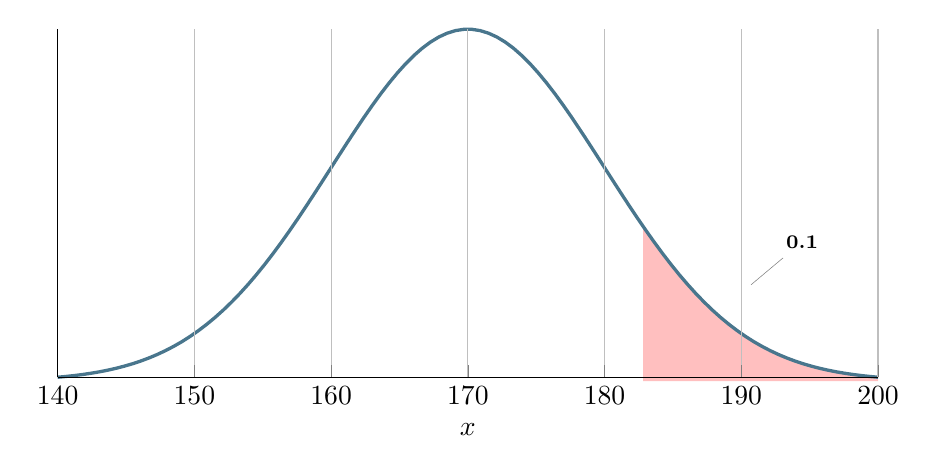
\begin{tikzpicture}
    \begin{axis}[
        no markers, 
        domain=-3:3, 
        samples=100, 
        axis lines*=left, 
        xlabel=$x$, 
        height=6cm, 
        width=12cm, 
        xtick={-3,-2,-1,0,1,2,3}, 
        xticklabels={140, 150, 160, 170, 180, 190, 200},
        ytick=\empty,
        enlargelimits=false, 
        clip=false, 
        axis on top,
        grid = major
    ]
    \addplot [very thick,cyan!50!black] {exp(-x^2/2)/sqrt(2*pi)};
    \addplot [name path=A,domain=1.282:3,cyan!50!black] {exp(-x^2/2)/sqrt(2*pi)};
    \path [name path=B] (axis cs:1.282,0) -- (axis cs:3,0);
    \addplot [red!50,opacity=0.5] fill between[of=A and B];
    \node[pin=above right:{\scriptsize \textbf{0.1}}] at (axis cs:2,0.1) {};
    \end{axis}
\end{tikzpicture}
\end{document}
